\subsection{Teoría de Grafos}

\subsubsection{¿Qué es la teoría de grafos?}

La teoría de grafos es una rama de las matemáticas que estudia las propiedades de sistemas complejos modelados mediante estructuras matemáticas llamadas \textbf{grafos}. Estas estructuras se utilizan para representar relaciones entre objetos. 

Un grafo está compuesto por:

\begin{itemize}
    \item Nodos: representan los objetos individuales.
    \item Enlaces: representan relaciones o conexiones entre los objetos.
\end{itemize}

Esta teoría tiene aplicaciones fundamentales en informática (redes de computadoras), biología (como redes metabólicas o neuronales), y especialmente en inteligencia artificial, se utiliza para modelar redes neuronales.

\paragraph{Origen histórico.}  
La teoría de grafos se originó en 1736 con el trabajo de Leonard Euler sobre el problema de los puentes de Königsberg. Este fue el primer problema formalizado usando un grafo y marcó el inicio de esta área.

\subsubsection{Problema principal}

El objetivo principal de la teoría de grafos es representar, analizar y resolver relaciones entre pares de elementos. Algunos problemas clásicos incluyen:

\begin{itemize}
    \item \textbf{Camino más corto:} ¿Cuál es la ruta más eficiente entre dos nodos?
    \item \textbf{Conectividad:} ¿Qué nodos están conectados entre sí directa o indirectamente?
    \item \textbf{Flujo en redes:} ¿Cuál es la máxima cantidad de flujo (información, energía, etc.) que se puede transmitir de un nodo a otro?  
        \begin{itemize}
            \item Se modela asignando capacidades a los enlaces y utilizando algoritmos como Ford-Fulkerson.
        \end{itemize}
    \item \textbf{Detección de ciclos y árboles:}  
        \begin{itemize}
            \item \textbf{Ciclo:} Secuencia de enlaces que comienza y termina en el mismo nodo.
            \item \textbf{Árbol:} Grafo conexo sin ciclos, que conecta todos los nodos con el mínimo número de enlaces (\(n-1\) para \(n\) nodos).
        \end{itemize}
\end{itemize}

\subsubsection{Conceptos clave}

\begin{center}
\begin{tabular}{@{}ll@{}}
\toprule
\textbf{Concepto} & \textbf{Descripción} \\
\midrule
\textbf{Grafo dirigido} & Los enlaces tienen una dirección (de un nodo a otro). \\
\textbf{Grafo no dirigido} & Los enlaces no tienen dirección, la relación es mutua. \\
\textbf{Camino} & Secuencia de nodos conectados por enlaces. \\
\textbf{Ciclo} & Camino cerrado donde el nodo inicial y final coinciden. \\
\textbf{Grado (degree)} & Número de enlaces conectadas a un nodo (grado de entrada y salida si es dirigido). \\
\textbf{Conectividad} & Existencia de caminos entre nodos en el grafo. \\
\textbf{Subgrafo} & Cualquier subconjunto de nodos y enlaces que forma un grafo. \\
\textbf{Árbol} & Grafo conexo sin ciclos. Si tiene \(n\) nodos, tiene \(n-1\) enlaces. \\
\bottomrule
\end{tabular}
\end{center}
\begin{figure}[H]
\centering
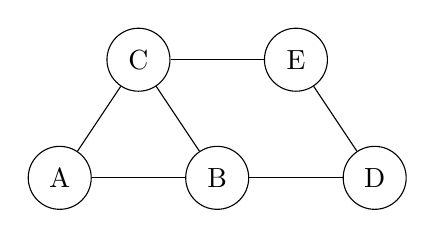
\begin{tikzpicture}[every node/.style={circle, draw, minimum size=0.8cm}, node distance=2cm]
    \node (A) at (0,0) {A};
    \node (B) at (2,0) {B};
    \node (C) at (1,1.5) {C};
    \node (D) at (4,0) {D};
    \node (E) at (3,1.5) {E};

    \draw (A) -- (B);
    \draw (B) -- (C);
    \draw (C) -- (A);
    \draw (B) -- (D);
    \draw (D) -- (E);
    \draw (E) -- (C);
\end{tikzpicture}
\caption{Ejemplo de grafo no dirigido. Contiene un ciclo entre A, B y C.}
\end{figure}

\begin{figure}[H]
\centering
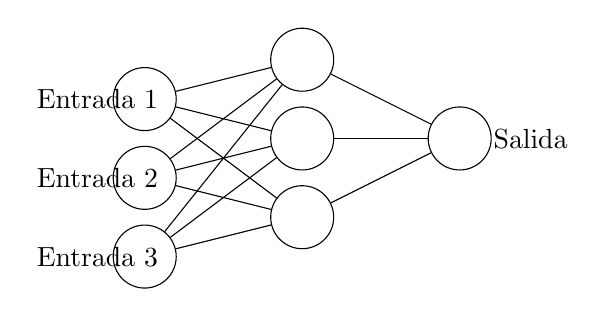
\begin{tikzpicture}[
    neuron/.style={circle, draw, minimum size=0.8cm},
    every edge/.style={draw, ->, >=Latex},
    node distance=1.5cm and 1.5cm,
    align=center
]

% Input layer
\node[neuron] (I1) at (0,2) {};
\node[neuron] (I2) at (0,1) {};
\node[neuron] (I3) at (0,0) {};

% Hidden layer
\node[neuron] (H1) at (2,2.5) {};
\node[neuron] (H2) at (2,1.5) {};
\node[neuron] (H3) at (2,0.5) {};

% Output layer
\node[neuron] (O1) at (4,1.5) {};

% Connections
\foreach \i in {1,2,3}
  \foreach \h in {1,2,3}
    \draw (I\i) -- (H\h);

\foreach \h in {1,2,3}
    \draw (H\h) -- (O1);

% Labels
\node at (-0.6,2) {Entrada 1};
\node at (-0.6,1) {Entrada 2};
\node at (-0.6,0) {Entrada 3};

\node at (4.9,1.5) {Salida};

\end{tikzpicture}
\caption{Red neuronal representada como grafo dirigido.}
\end{figure}

\subsubsection{Métricas estadísticas y estructurales}

Estas métricas permiten analizar cuantitativamente las propiedades del grafo. Son esenciales para entender su estructura global y la importancia de sus componentes.

\begin{center}
\begin{tabular}{@{}lp{10.5cm}@{}}
\toprule
\textbf{Métrica} & \textbf{Significado} \\
\midrule
\textbf{Grado medio} (\( \langle k \rangle \)) & Promedio de conexiones por nodo. \\
\textbf{Distribución de grados} & Probabilidad de que un nodo tenga cierto número de conexiones. \\
\textbf{Centralidad} & Mide la importancia de un nodo. Tipos: 
\begin{itemize}
    \item \textbf{Degree centrality:} número de conexiones.
    \item \textbf{Closeness:} inverso de la distancia promedio al resto.
    \item \textbf{Betweenness:} cuántos caminos más cortos pasan por el nodo.
\end{itemize} \\
\textbf{Diámetro} & Máxima distancia (camino más corto) entre dos nodos cualesquiera. \\
\textbf{Longitud promedio del camino} & Promedio de distancias más cortas entre todos los pares de nodos. \\
\textbf{Densidad} & Relación entre el número de enlaces existentes y el número máximo posible. \\
\textbf{Coeficiente de agrupamiento} & Mide cuán conectados están los vecinos de un nodo (transitividad local). \\
\bottomrule
\end{tabular}
\end{center}

\subsubsection{Aplicación a redes neuronales}

Las redes neuronales artificiales pueden modelarse como grafos dirigidos con peso:

\begin{itemize}
    \item Las \textbf{neuronas} son los \textbf{nodos} del grafo.
    \item Las \textbf{conexiones sinápticas} son los \textbf{enlaces dirigidos} con un \textbf{peso} asociado, que representa la fuerza de la conexión.
\end{itemize}

Este enfoque permite aplicar herramientas de teoría de grafos para analizar, optimizar y entender el comportamiento estructural de las redes neuronales.

\subsubsection*{Ejemplos de aplicaciones}

\begin{itemize}
    \item \textbf{Visualización y análisis estructural:} identificar cuellos de botella, redundancias y zonas críticas.
    \item \textbf{Análisis de capas:} usando conectividad, centralidad y otras métricas para caracterizar cada capa de la red.
    \item \textbf{Redes neuronales recurrentes (RNN):} se modelan naturalmente como grafos con ciclos, debido a su retroalimentación temporal.
    \item \textbf{Interpretabilidad:} detectar nodos influyentes o rutas críticas usando centralidades y flujo.
    \item \textbf{Graph Neural Networks (GNN):} modelos de aprendizaje profundo que operan directamente sobre estructuras de grafos, utilizados en química computacional, redes sociales, procesamiento de lenguaje natural, entre otros.
\end{itemize}
